\chapter{Using Wave-DNA}
\label{chap:Using Wave-DNA}



\section{Installation}
\label{sec:Installation}

\begin{compactitem}
\item {\tt CMakeLists.txt}
\item {\tt cleanbuild\_release.sh}
\item {\tt cleanbuild\_debug.sh}
\end{compactitem}
It is convenient to compile the source code in a build directory separate from the source directory by executing the {\tt cleanbuild\_release.sh} script to compile in optimized release mode, or by excecuting the {\tt cleanbuild\_debug.sh} script to compile in debug mode. The program runs significantly faster in release mode.

By running the build scripts ({\tt cleanbuild\_release.sh} or {\tt cleanbuild\_debug.sh}), all files in the build directory that were previously generated by {\tt cmake} are removed. Subsequently, a {\tt cmake} run is performed on the {\tt CMakeLists.txt} file. In the {\tt CMakeLists.txt} file, the {\tt gcc} compiler must be set as {\tt CMAKE\_C\_COMPILER}, providing the path to the {\tt gcc} executable. For instance:
\\[8pt]
{\tt set(CMAKE\_C\_COMPILER /usr/bin/gcc)}
\\[8pt]
Furthermore, the environmental variable  {\tt \${mylibdirs}} must be set in {\tt CMakeLists.txt}. For instance:
\\[8pt]
{\tt set(mylibdirs \${mylibdirs} /usr/lib64/)}
\\[8pt]
Finally, the {\tt Wave-DNA} source directory must be specified. This is done by either directly setting the path to the source directory as
\\[8pt]
{\tt FILE (GLOB\_RECURSE MYFILES ABSOLUTE  /path/to/wavedna/src/*.c)}
\\[8pt]
or by setting:
\\[8pt]
FILE (GLOB\_RECURSE MYFILES ABSOLUTE  \$ENV{APECSS\_DIR}/src/*.c)
\\[8pt]
The latter option requires to set the environmental variable {\tt \$ENV{APECSS\_DIR}} to {\tt /path/to/wavedna} in the configuration (run commands) file of the {\tt Unix} shell, as for instance {\tt /path/to/home/.bashrc}. With the default settings in the delivered {\tt CMakeLists.txt} file, the executable {\tt WaveDNA} is created in the build directory upon successful compilation. See the following lines in 
\\[8pt]
{\tt add\_executable(WaveDNA \${MYFILES})} \\
{\tt target\_link\_libraries(WaveDNA \${mylibs}}
\\[8pt]


\section{Running a simulation}
\label{sec:Running a simulation}

The simulation case directory must contain a folder {\tt results}, in which the output files are written, and an options file file called {\tt run.DNA}, which contains the user options. The simulation is run in the case directory by executing the following command:
\\[8pt]
{\tt /path/to/some/arbitrary/build/directory/WaveDNA}
\\[8pt]
The case directories must contain the following files and sub-directories:
\begin{compactitem}
\item {\tt run.DNA}: This is the options file as further explained in Sec. \ref{sec:Run options and fluid properties}. If the file is empty, a default run is performed based on the default options as indicated in Sec. \ref{sec:Default settings} (also see {\tt src/io/iodefaultoptions.c}).
\item {\tt results}: This is the sub-directory in which the output files (see Sec. \ref{sec:Results}) are written. If an output already exists, it will be appended. Therefore, existing output files should be deleted/moved prior to the start of the simulation if a clean start is desired.
\end{compactitem}



\section{Run options and fluid properties}
\label{sec:Run options and fluid properties}

The basic run options and fluid properties are set in the sections {\tt RUNOPTIONS} and {\tt FLUID}, respectively. Next to the background density and speed of sound, $\rho_0$ and $c_0$, respectively, one can specify the nonlinearity coefficient $\beta$ to admit cumulative nonlinearities. Independent of this option, one can further indicate, whether local nonlinearties (a non-zero Lagrangian density $\mathcal{L}$) are taken into account. By this means, one can effectively solve 
\begin{compactitem}
\item the linear wave equation ($\beta = 0$, $\mathcal{L}=0$),
\item the lossless Westervelt equation ($\beta \neq 0$, $\mathcal{L}=0$),
\item or the lossless Kuznetsov equation ($\beta \neq 0$, $\mathcal{L}\neq 0$).
\end{compactitem}
The following table provides a detailed overview of the run and fluid property options.

\noindent
\begin{longtable}{p{0.4\textwidth} p{0.55\textwidth}}
\textbf{Command} & \textbf{Description} 
\vspace{1mm} \\
\hline Section {\tt RUNOPTIONS} &\\ \hline
{\tt TimeStart <float>} & Physical start time of the simulation. \\ 
{\tt TimeEnd <float>} & Physical end time of the simulation. \\{\tt WriteFrequency <float>} & Number of time steps between successive write to disc occurrences. This determines the time instances at which the field data is written to disc (fields.dat). The data recorded at sample points is stored in buffer and written to disc (probes.dat) at this occasion as well. \\  
{\tt SamplePoints <int> <float> ...} & Number of sample points ({\tt <int>}) followed by the coordinates ({\tt <float>}) of the sample points. The nearest neighbour grid points to the target locations and their IDs is identified and the sample is taken at those grid points throughout the entire simulation. This means that the probe is moving with the grid. If the indicated number of sample points is larger than zero and does not match the number of given points, the simulation aborts with the error message "{\tt An unknown option ...}". \\
\\
\hline Section {\tt FLUID} &\\ \hline
{\tt SoundSpeed <float>} & Background speed of sound $c_0$ of the fluid. \\ 
{\tt Density <float>} & Background density $\rho_0$ of the fluid. \\ 
{\tt FluidNonLinearity <float>} & Nonlinearity coefficient $\beta$ of the fluid. \\
{\tt LocalNonlinearity <string>} & If set to {\tt True}, the second-order acoustic terms giving rise to local nonlinear wave propagation are active. The option {\tt False} (default) in combination with a non-zero value for $\beta$ effectively means that the Westervelt equation is solved. \\
 \hline
\end{longtable} \vspace{1em}


\section{Wave excitation}
\label{sec:Wave excitation}

Several options are available to excite an acoustic pressure wave at a specific emission node. The present modeling framework is particularly designed to solve boundary value problems, where the domain boundaries act as wave-emitting boundaries. Before explaining the the different types of excitation functions, there some important remarks:

\begin{compactitem}
\item The moving boundary is always associated with the grid node 0, regardless of whether its coordinate $R\left(t\right)$ takes a larger or smaller value than the coordinate $R_{\mathrm{stat}}$ of the fixed boundary. This particular feature is illustrated in Fig. \ref{fig:domain3}, where the positive direction of the $r$-axisof the physical domain $\Omega\left(t\right)$ relative to the positive direction of the $\xi$-axis of the computational domain $\Theta$ depends on whether $R<R_{\mathrm{stat}}$ or $R>R_{\mathrm{stat}}$. This means that the grid node $N_{\mathrm{points}}-1$ is always associated with the fixed boundary $R_{\mathrm{stat}}$.  
\item Only one single excitation can be specified in the present version.
\item One is free to specify any node between $0$ and $N_{\mathrm{points}}-1$. However, as the present modeling framework is specifically designed to solve boundary value problems, the source pressure is not a volumetric source.
\item The emission of the acoustic pressure as specified by the excitation function is always strictly enforced as per applied boundary condition, regardless of whether the wave-emitting boundary is in relative motion to the background medium or not. Consequently, the effect of convective amplification/attenuation, which relies on the Doppler-factor of the relative motion between emitter and background medium \citep{Ostashev_et_al_2005}, must be taken into account in the specification of the emitted acoustic pressure amplitude. 
\end{compactitem}

The sinusoidal excitation function for the acoustic pressure $p_1$ at the emission node is given by
\begin{equation}
\left.p_1\left(t\right)\right|_{\mathrm{emission\:node}} = G\left(t\right)\Delta p_{\mathrm{a}}\left[\sin\left(2\pi f_{\mathrm{a}}t - \Delta \varphi\right)\right]^n,
\label{eq:ExcitationSine}
\end{equation}
where $\Delta p_{\mathrm{a}}$, $f_{\mathrm{a}}$, and $\Delta \phi$ are the emitted acoustic pressure amplitude, the excitation frequency and a fixed phase-shift, respectively. The sine can be raised can be raised to a power $n$ in order to admit nonlinearities in the excitation signal. The factor $G\left(t\right)$ is a Gauss function given by
\begin{equation}
\left.G\left(t\right)\right|_{\mathrm{emission\:node}} = q^{\displaystyle\left[ 4\left(f_{\mathrm{a}}t - N + 1/2\right)^2\right]},
\label{eq:GaussEnvelope}
\end{equation}
which has a peak value of unity and where $q$ is a shape coefficient that specifies the width of the Gaussian. Eq. \eqref{eq:GaussEnvelope} can be used in conjunction with Eq. \eqref{eq:ExcitationSine} in order to obtain a Gauss-enveloped sinusoidal excitation signal, where Gaussian peaks at the center of the $N^{\textnormal{th}}$ period Alternatively, it can be used to emit a Gaussian Pulse $\Delta p_{\mathrm{a}}G\left(t\right)$, where $f_{\mathrm{a}}$ and $N$ as well $\Delta _{\mathrm{a}}$ must be specified to indicate the center time and the amplitude of the pulse, respectively. The parameters of Eqs. \eqref{eq:ExcitationSine} and \eqref{eq:GaussEnvelope} are set in the section {\tt EXCITATION} as follows.

\noindent
\begin{longtable}{p{0.4\textwidth} p{0.55\textwidth}}
\textbf{Command} & \textbf{Description} 
\vspace{1mm} \\
\hline Section {\tt EXCITATION} &\\ \hline
{\tt ExcitationStart <float>} & Physical start time of the wave excitation, equal to the simulation start time {\tt TimeStart} per default (see {\tt RUNOPTIONS}). \\ 
{\tt ExcitationEnd <float>} & Physical end time of the wave excitation, equal to the simulation end time {\tt TimeEnd} per default (see {\tt RUNOPTIONS}). \\
{\tt ExcitationNode <int>} & Node (ID of the grid point) at which the wave is excited (0 is default). \\  
{\tt ExcitationFunctionType <string>} & Type of the excitation function. Options are {\tt sine} (Eq. \eqref{eq:ExcitationSine}) and {\tt GaussPulse}. The latter is given by Eq. \eqref{eq:GaussEnvelope} times the pressure amplitude specified below. \\
{\tt PressureAmplitude <float>} & Excitation amplitude $\Delta p_{\mathrm{a}}$ of the acoustic pressure signal $p_1$. This applies to both the options {\tt sine} and {\tt GaussPulse}. \\
{\tt ExcitationFrequency <float>} & Unmodulated frequency $f_{\mathrm{a}}$ of the excitation signal if {\tt ExcitationFunctionType} is set to {\tt sine}. \\
{\tt PhaseShiftAngle <float>} & Phase shift angle $\Delta \varphi$ in the argument of the excitation signal if {\tt ExcitationFunctionType} is set to {\tt sine}. \\
{\tt PowerCoeff <float>} & The sinusoidal excitation function ({\tt sine} must be set for {\tt ExcitationFunctionType}) can be raised to a power $n$ (1.0 is default).\\
{\tt GaussEnvelope <string>} & The excitation function can be enveloped by the Gauss function $G\left(t\right)$ with peak value 1.0 by setting this option to {\tt True} ({\tt False} is default). If {\tt ExcitationFunctionType} is set to {\tt GaussPulse}, the corresponding pointer is set to a function that returns the amplitude of the excitation signal ({\tt PressureAmplitude}), which is then convoluted by the Gauss function, irrespective of the option for {\tt GaussEnvelope <string>}. \\
{\tt EnvelopedPeriod <float>} & Period number $N$ of the sinusoidal excitation function that is Gauss-enveloped by Eq. \eqref{eq:GaussEnvelope} (not necessarily an integer). This setting can also be used to specify the center of the peak in the time domain if {\tt ExcitationFunctionType} is set to {\tt GaussPulse}.\\
{\tt GaussShapeCoeff <float>} & Coefficient $q$ in Eq. \eqref{eq:GaussEnvelope} that determines the width of the Gauss pulse in the time domain. \\
\hline
\end{longtable} \vspace{1em}

\begin{figure}
\centering
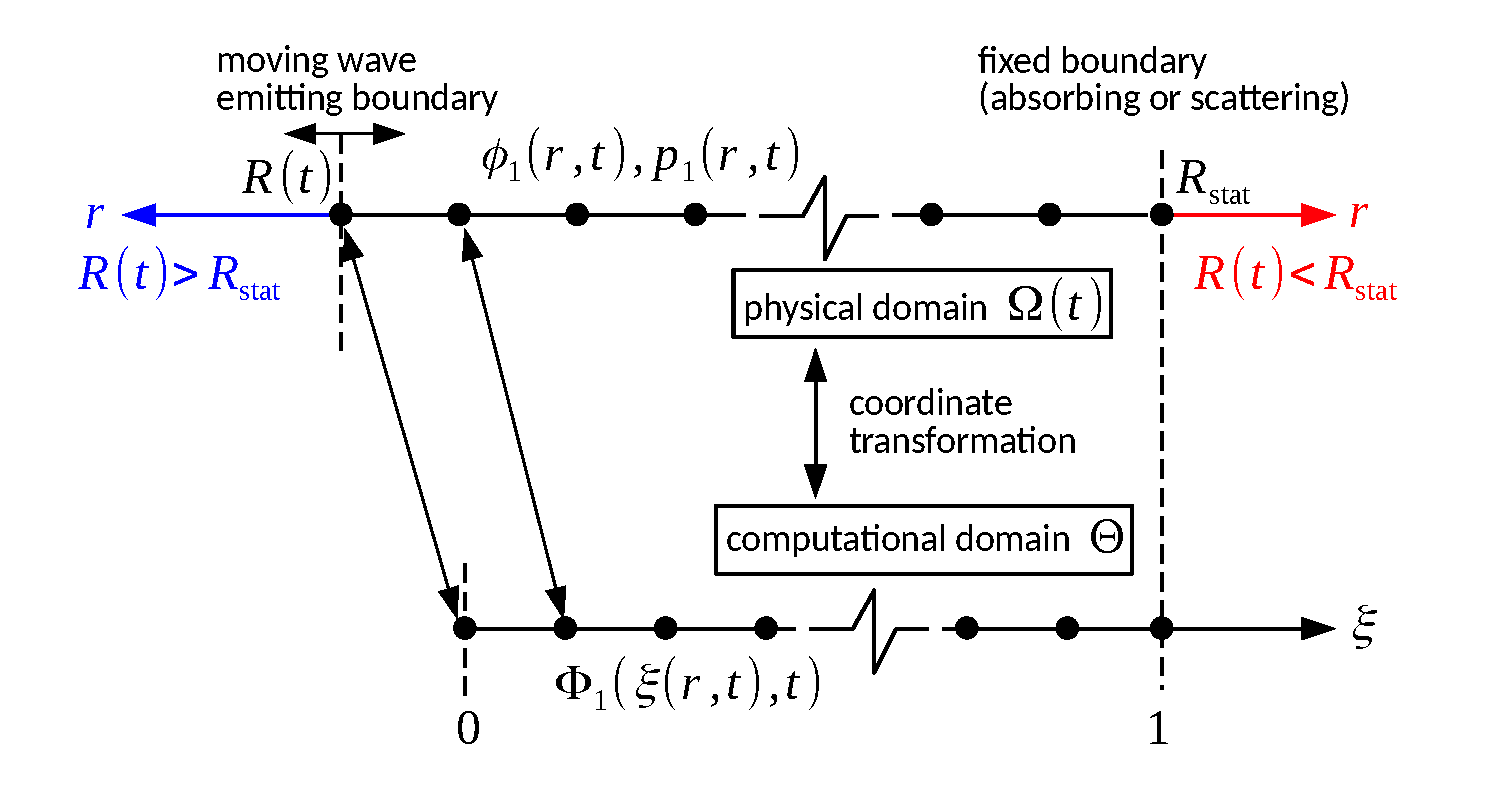
\includegraphics[width=0.7\textwidth]{figures/domain3.pdf}
\caption{Illustration of the physical domain $\Omega\left(t\right)$ with moving wave-emitting boundary $R\left(t\right)$ and fixed boundary $R_{\mathrm{stat}}$, and the fixed computational domain $\Theta$.}
\label{fig:domain3}
\end{figure}




\section{Boundary, grid, and background flow motion}
\label{sec:Boundary, grid, and background flow motion}

The present simulation framework for moving domain boundaries and background flow fields admits the following configurations, where one boundary is always fixed whereas the other can be either fixed or moving:
\begin{compactitem}
\item \textbf{Moving emitter/scatterer in a quiescent medium:} One of the domain boundaries is in motion whereas the background medium is at rest. This configurations gives rise to the classical Doppler shift. If the moving boundary is the wave emitting boundary, it acts like a moving wave emitter. If the non-moving boundary is the wave emitting boundary, the moving boundary acts like a moving wave scatterer, given the corresponding boundary condition is not an absorbing one.
\item \textbf{Moving flow inducing boundary:} The moving boundary induces a background flow field by mimicking a solid boundary that displaces the surrounding fluid. The wave may be emitted by the moving boundary itself, so that the emitter does not move relative to the background flow field. Alternatively, the wave may be excited at the fixed boundary (or any node between the left and the right boundary), so that emitter and background medium are in relative motion.
\item \textbf{Stationary acoustic black/white hole:} A special case of the previous configuration is the acoustic black or white hole. In principle, any of the options to specify the boundary and fluid motion can mimic a background flow field with sonic transition. However, the framework specifically allows to simulate stationary spherical acoustic black holes and white holes with a pre-defined radius of the sonic horizon.
\item \textbf{Linear vs nonlinear acoustics:} All of the above options can be combined with the assumption of linear acoustics ($\beta=0$, $\mathcal{L}=0$), or with nonlinear acoustics as specified in Sec. \ref{sec:Run options and fluid properties}. 
\end{compactitem}

The background flow velocity distribution is either spatially uniform in the case of a one-dimensional Cartesian geometry (it may still be time-dependent if one of the boundaries is moving), or it follows the relation
\begin{equation}
u_0\left(r,t\right) = \dot R\left(t\right)\left(\dfrac{R\left(t\right)}{r}\right)^n,
\label{eq:u0_spherical}
\end{equation}
in a spherically symmetric configuration. In the present implementation, the parameter $n$ is a constant equal to 2 per default, such that Eq. \eqref{eq:u0_spherical} represents the spherically symmetric velocity field obeying the continuity equation for an incompressible flow field. The value of $n$ may be changed in the options file, and with some minor modifications of the source, even time- and space-dependent distributions of $n$ can be realized. However, if considerable Mach numbers are involved, it should be noted that according to the theory underpinning the present modeling framework, the background density and speed of sound are assumed to be constants as well. Therefore, the background fluid state obtained for the acoustic black hole scenario represents a so called slab geometries rather than a fully physical configuration. 


It follows from the linear coordinate transformation
\begin{equation}
\xi\left(r,t\right) = \mathcal{X}_{\infty} + \left(r - R_{\mathrm{stat}}\right) \dfrac{\mathcal{X}_{\mathrm{\infty}} - \mathcal{X}_{R}}{R_{\mathrm{stat}}-R\left(t\right)}
\label{eq:linTrans}
\end{equation}
that
\begin{align}
& \dfrac{\partial \xi}{\partial r} = \dfrac{\mathcal{X}_{\mathrm{\infty}} - \mathcal{X}_{R}}{R_{\mathrm{stat}}-R\left(t\right)},
\label{eq:linJacobian} \\[4pt]
& \dfrac{\partial \xi}{\partial t} = 
-\dfrac{\mathcal{X}_{\mathrm{\infty}} - \xi}{R_{\mathrm{stat}} - R\left(t\right)} \dot R\left(t\right),<
\label{eq:linq}
\\[4pt]
& \dfrac{\partial^2 \xi}{\partial t \partial \xi} = \dfrac{\dot R\left(t\right)}{R_{\mathrm{stat}} - R\left(t\right)},
\label{eq:lindivq} \\[4pt]
& \dfrac{\partial^2 \xi}{\partial r \partial \xi} = 0,
\label{eq:linJacobiandxi} \\[4pt]
& \dfrac{\partial^2 \xi}{\partial t^2} = 2\dfrac{\partial \xi}{\partial t}\dfrac{\partial^2\xi}{\partial t\partial \xi} - \ddot R\dfrac{\partial \xi}{\partial r} \dfrac{\mathcal{X}_{\infty} - \xi}{\mathcal{X}_{\infty} - \mathcal{X}_{R}}.
\label{eq:lindqdt}
\end{align}
The motion of the grid-points is then fully described by instantaneous position $R$ of the moving domain boundary and the velocity $\dot R$ and acceleration $\ddot R$ thereof. In the case of linear boundary motion, $R=\mathrm{const}$ so that $\dot R=0$ and $\ddot R=0$. An oscillatory boundary motion is described by the function
\begin{align}
& R\left(t\right) = R_0 + \dfrac{\Delta v_{\mathrm{b,a}}}{2\pi f_{\mathrm{b}}}\sin\left(2\pi f_{\mathrm{b}}t\right)
\label{eq:oscillatingBoundary_R}, \\[4pt]
& \dot R\left(t\right) = \Delta v_{\mathrm{b,a}}\cos\left(2\pi f_{\mathrm{b}}t\right)
\label{eq:oscillatingBoundary_dotR}, \\[4pt]
& \ddot R\left(t\right) = -2\pi f_{\mathrm{b}}\Delta v_{\mathrm{b,a}}\sin\left(2\pi f_{\mathrm{b}}t\right)
\label{eq:oscillatingBoundary_ddotR},
\end{align}
where $f_{\mathrm{b}}$ and $\Delta v_{\mathrm{b,a}}$ are the frequency and the velocity amplitude of the oscillating boundary, respectively. With $r_{\mathrm{h}}$ being the steady-state sonic horizon radius in a flow field obeying Eq. \eqref{eq:u0_spherical}, the functions describing the boundary motion are given by
\begin{align}
& R\left(t\right) = \left[R_0^{n+1} - \left(n+1\right)c_0r_{\mathrm{h}}^nt\right]^{\frac{1}{n+1}},
\label{eq:R} \\[4pt]
& \dot R\left(t\right) = -c_0r_{\mathrm{h}}^n\left[R_0^{n+1} - \left(n+1\right)c_0r_{\mathrm{h}}^nt\right]^{-\frac{n}{n+1}},
\label{eq:Rdot} \\[4pt]
& \ddot R\left(t\right) = -nc_0^2r_{\mathrm{h}}^{2n}\left[R_0^{n+1} - \left(n+1\right)c_0r_{\mathrm{h}}^nt\right]^{-\frac{2n+1}{n+1}}
\label{eq:Rddot}
\end{align}
for the acoustic black hole scenario, and by 
\begin{align}
& R\left(t\right) = \left[R_0^{n+1} + \left(n+1\right)c_0r_{\mathrm{h}}^nt\right]^{\frac{1}{n+1}},
\label{eq:R_WH} \\[4pt]
& \dot R\left(t\right) = c_0r_{\mathrm{h}}^n\left[R_0^{n+1} + \left(n+1\right)c_0r_{\mathrm{h}}^nt\right]^{-\frac{n}{n+1}},
\label{eq:Rdot_WH} \\[4pt]
& \ddot R\left(t\right) = -nc_0^2r_{\mathrm{h}}^{2n}\left[R_0^{n+1} + \left(n+1\right)c_0r_{\mathrm{h}}^nt\right]^{-\frac{2n+1}{n+1}}
\label{eq:Rddot_WH}
\end{align}
for the acoustic white hole scenario.

\noindent
\begin{longtable}{p{0.4\textwidth} p{0.55\textwidth}}
\textbf{Command} & \textbf{Description} 
\vspace{1mm} \\
\hline Section {\tt BOUNDARYMOTION} &\\ \hline
{\tt BoundaryMotionType <string>} & Function type describing the motion of the moving domain boundary. Options are {\tt <linear>} for a constant velocity, {\tt <oscillating>} for an oscillatory motion around the initial position, described by a sine function (see Eq. \eqref{eq:oscillatingBoundary_R}), and {\tt <stationaryBlackHole>} as well as {\tt <stationaryWhiteHole>} for the simulation of a stationary sonic horizon in acoustic black black hole or white hole configurations (see Eq. \eqref{eq:R}). \\
{\tt BoundaryMotionStartTime <float>} & Physical time $t_{\mathrm{boundary\:start}}$ at which the moving boundary starts to move from its intial position. The function describing the boundary motion depends on the time $t-t_{\mathrm{boundary\:start}}$. \\
{\tt BoundaryMotionEndTime <float>} & Physical time at which the boundary motion ends. The boundary position will remain constant for the remaining simulation time. \\ 
{\tt InitialMovingBoundaryPosition <float>} & Initial position of the moving domain boundary, where 0.0 is default. \\
{\tt FixedBoundaryPosition <float>} & Position of the fixed domain boundary. The default setting is a domain that comprises ten emitted wavelengths $\lambda_0=c_0/f_{\mathrm{a}}$ based on the given or the default {\tt InitialMovingBoundaryPosition}. \\
{\tt MovingBoundaryVelocityAmplitude <float>} & Velocity amplitude $\Delta v_{\mathrm{b,a}}$ of the moving domain boundary if {\tt BoundaryMotionType} is set to {\tt <oscillating>}. If {\tt BoundaryMotionType} is set to {\tt <linear>}, $\lambda_0=c_0/f_{\mathrm{a}}$ represents the constant boundary velocity. \\
{\tt MovingBoundaryFrequency <float>} & Frequency $f_{\mathrm{b}}$ of the moving domain boundary if {\tt BoundaryMotionType} is set to {\tt <oscillating>}, where $f_{\mathrm{b}} = 0.1f_{\mathrm{a}}$ is default. \\
\\
\hline Section {\tt BACKGROUNDFLOW} &\\ \hline
{\tt BackgroundMotionMode <string>} & Specifies whether the background flow field is unconditionally quiescent (option {\tt <quiescent>}), regardless of the motion of the moving domain boundary, or whether the background flow field is coupled to the moving domain boundary (option {\tt <coupledToMovingBoundary>}). \\
{\tt Geometry <string>} & Specifies whether the flow field is spatially homogeneous (option {\tt <1dCartesian>}) or satisfying the continuity equation of a spherically symmetric flow (option {\tt <3dSphericallySymmetric>}). \\ 
{\tt HorizonRadius <float>} & Point of sonic transition if {\tt BoundaryMotionType} is set to {\tt <stationaryHorizon>}. \\ 
{\tt GravitationalPotential <string>} & If set to {\tt True} and if {\tt BackgroundMotionMode} is set to {\tt <stationaryHorizon>}, a gravitational potential is included to mimic a simplified Bondi-Parker-type flow. \\ 
 \hline
\end{longtable} \vspace{1em}


\section{Finite difference discretization}
\label{sec:Finite difference discretization}

To be compatible with the predictor-corrector method and the wave-absorbing boundary conditions as explained further below, we use first-order finite differences in time. For the spatial discretization, second-order central differences are used. The Laplacian and the mixed spatial-temporal derivatives only need to be evaluated in the inner field, whereas the gradient also needs to be evaluated at the boundary in order to impose the wave-absorbing boundary condition. At the boundaries, a first-order finite difference stencil is used to compute the gradient. The Courant-Friedrichs-Lewy number is given by
\begin{equation}
\mathrm{CFL} = \dfrac{c_0\Delta t}{\Delta x} = \dfrac{c_0\Delta t\left(N_{\mathrm{points}-1}\right)}{L_{\mathrm{domain}}},
\label{eq:CFL}
\end{equation}
where $\Delta t$ and $\Delta x$ are the time-step size and the spatial step size, respectively, and $N_{\mathrm{points}}$ and $L_{\mathrm{domain}}$ are the total number of grid points in the domain, including the boundaries, and the length of the physical domain, respectively.

Next to the time step size $\Delta t$ and the total number of grid points, one can specify the parameter $\gamma$ of a predictor-corrector method as developed by \citet{Dey_and_Dey_1983} and \citet{Nascimento_et_al_2010}, where the interim solution $\widetilde{\Phi_1}$, predicted by the explicit finite difference integration, is given the weight the weight $\left(1-\gamma\right)$, whereas the corrected solution is weighted by $\gamma$. With $i$ and $j$ indicating the grid point and the time step, respectively, the spatial and temporal finite difference approximations are given by
\begin{align}
&\left(\dfrac{\partial^k \Phi_1}{\partial t^k}\right)^{j}_{i}
=
\dfrac{a_0^{\left(k\right)}}{\Delta t^k} \Phi^{j+1}_{1,i}
+
\dfrac{1}{\Delta t^k}\underbrace{\sum_{n=1}^{N-1} a_n^{\left(k\right)}\Phi^{j+1-n}_{1,i}
}_{b^{\left(k,j\right)}_i},
\label{eq:fddt_compact} \\
& \left(\dfrac{\partial^k \Phi_1}{\partial \xi^k}\right)^{j}_{i}
=
\dfrac{\displaystyle a_0^{\left(k\right)}\Phi^{j}_{1,i} + \sum_{n=1}^{\left(N-1\right)/2} \left( a_n^{\left(k\right)}\Phi^{j}_{1,i+n} + a_{n}^{\left(k\right)}\Phi^{j}_{1,i-n}\right)}{\Delta\xi^k}.
\label{eq:fddxi_compact}
\end{align}
The predicted solution $\widetilde{\Phi_{1,i}}$ is obtained as
\begin{equation}
\widetilde{\Phi_{1,i}}\underbrace{\sum_{k=1}^2\mathcal{A}_{k,i}^j \dfrac{a_0^{\left(k\right)}}{\Delta t^k}}_{\mathcal{H}^j_i}
+
\underbrace{\mathcal{R}^j_i
+
\sum_{k=1}^2\mathcal{A}_{k,i}^j \dfrac{b^{\left(k,j\right)}_i}{\Delta t^k}}_{\mathcal{S}^j_i}
=
- \mathcal{A}^j_{L,i}\left(\dfrac{\partial^2 \Phi_1}{\partial \xi^2}\right)^j_i + \left(\dfrac{c_0^2}{A}\dfrac{\partial A}{\partial r} \dfrac{\partial \xi}{\partial r}\right)^j_i\left(\dfrac{\partial \Phi_1}{\partial \xi}\right)^,
\label{eq:discreteEqn}
\end{equation}
where the term $\mathcal{R}_i^j$ involves the finite difference approximations of the gradient and mixed derivative terms. The new solution $\Phi^{j+1}_{1,i}$ is then obtained as
\begin{equation}
\Phi^{j+1}_{1,i} = \left(1-\gamma\right)\widetilde{\Phi_{1,i}} + \dfrac{\gamma}{\mathcal{H}^j_i\left(\Phi_{1,i}^{j}\right)}\left[\underbrace{\mathcal{A}^j_{L,i}\left(\Phi_{1,i}^{j}\right)\left(\dfrac{\partial^2\widetilde{\Phi_1}}{\partial \xi^2}\right)_i - \left(\dfrac{c_0^2}{A}\dfrac{\partial A}{\partial r} \dfrac{\partial \xi}{\partial r}\right)^j_i\left(\dfrac{\partial \widetilde{\Phi_1}}{\partial \xi}\right)_i}_{\textnormal{spherical Laplacian}} + \mathcal{S}^j_i\left(\Phi_{1,i}^{j}\right)\right],
\label{eq:corrector}
\end{equation}
where the spherical Laplcian is updated based on the predicted solution $\widetilde{\Phi_1}$, whereas all remaining terms, summarized in the terms $\mathcal{H}$ and $\mathcal{S}$ and the time- and space-dependent coefficient $\mathcal{A}_L$, remain unchanged in the corrector step. The corrector step may be performed multiple times in a corrector loop. However, a single corrector step should serve the purpose of counteracting the dispersive noise. In fact, the value of $\gamma$ is more important. For $\gamma=0$, the standard exlicit finite difference time integration scheme is obtained. With increasing $\gamma$, the predictor-corrector method becomes increasingly diffusive. The resolution of the simulation must be increased at constant $\mathrm{CFL}$ number in order to avoid excessive diffusion while preserving the stabilizing effect of the scheme. In order words, the increase in numerical stability comes at the expense of an increased computational effort to preserve the accuracy of the numerical solution. Rather than representing a blended solution, the predictor-corrector method effectively generates a $\Delta x$- and $\Delta t$-dependent attenuation term \citep{Nascimento_et_al_2010} predominantly acting on the higher frequencies. Therefore, values of $\gamma \le 1$ are possible and may even be required, in particular if shocks are involved. The following table provides an overview of the options for the finite difference discretization.

The boundary conditions can either be scattering, where the incoming wave is fully reflected at the domain boundary, or absorbing, where the incoming wave passes the domain boundary without reflection. The absorbing boundary condition is based on Mur's first-order absorbing boundary condition, given by \citep{Mur_1981}
\begin{align}
& \Phi_{1,0}^{j+1} = \Phi_{1,1}^{j} + \dfrac{\mathrm{CFL-1}}{\mathrm{CFL}+1}\left(\Phi_{1,1}^{j+1}-\Phi_{1,0}^{j}\right)
+ 2u_{1,1}^{j}\dfrac{\Phi_{1,0}^{j} - \Phi_{1,N}^{j}}{\Delta x},
\label{eq:Mur_West} \\[4pt]
& \Phi_{1,N}^{j+1} = \Phi_{1,N-1}^{j} + \dfrac{\mathrm{CFL-1}}{\mathrm{CFL}+1}\left(\Phi_{1,N-1}^{j+1}-\Phi_{1,N}^{j}\right)
+ 2u_{1,N}^{j}\dfrac{\Phi_{1,N-1}^{j} - \Phi_{1,N}^{j}}{\Delta x}
\label{eq:Mur_East}
\end{align}
for the West and the East boundary, respectively, and where the advective terms are added in order to allow the waves to pass the domain boundaries in the presence of a non-zero background flow field.

\noindent
\begin{longtable}{p{0.4\textwidth} p{0.55\textwidth}}
\textbf{Command} & \textbf{Description} 
\vspace{1mm} \\ 
\hline Section {\tt FINITEDIFFERENCE} &\\ \hline
{\tt TimeStepSize <float>} & Constant time step size $\Delta t$, where the acoustic $\mathrm{CFL}$ number takes the value 0.1 per default. \\ 
{\tt NPoints <int>} & Total umber of grid points in the computational domain, including the domain boundaries, where the default setting is such that 100 points per emitted wavelength $\lambda_0 = c_0/f_{\mathrm{a}}$ are obtained based on the given or default domain size. \\ 
{\tt nCorrectors <int>} & Number of corrector steps applied in the predictor-corrector method to counteract the formation of dispersive numerical noise (1 per default). \\ 
{\tt correctorWeight <float>} & Corrector weight $\gamma$ to specify the weight of the corrected solution in the predictor-corrector method, where $\gamma\ge0$ and $\gamma=0.1$ per default.\\ 
{\tt BoundaryConditionEast <string>} & Boundary condition at the Eastern (right) domain boundary. Options are {\tt <scattering>} for wave-reflecting boundaries and {\tt <absorbing>} (default) for non-reflecting boundaries. \\  
{\tt BoundaryConditionWest <string>} & Boundary condition at the Western (right) domain boundary. Options are {\tt <scattering>} for wave-reflecting boundaries and {\tt <absorbing>} (default) for non-reflecting boundaries. \\  
\hline
\end{longtable} \vspace{1em}




\section{Default settings}
\label{sec:Default settings}

These are the default settings for the {\tt Wave-DNA} options file {\tt run.DNA}, indicating the dependencies between certain dafault settings (see the source file {\tt src/io/iodefaultoptions.c}). The default settings are used if the corresponding option is not included in {\tt run.DNA}.

{\tt
FLUID \\
SoundSpeed 1500.0 \\
Density 1000.0 \\
FluidNonLinearity 0.0 \\
LocalNonlinearity False \\
END \\

RUNOPTIONS \\
TimeStart 0.0 \\
TimeEnd 10.0/<ExcitationFrequency> \\
WriteFrequency (<TimeEnd> - <TimeStart>)/<TimeStepSize> \\
SamplePoints 0 \\
END

BOUNDARYMOTION \\
BoundaryMotionType linear \\
BoundaryMotionStartTime <TimeStart> \\
BoundaryMotionEndTime <TimeEnd> \\
InitialMovingBoundaryPosition 0.0 \\
FixedBoundaryPosition 10.0*<SoundSpeed>/<ExcitationFrequency> \\
MovingBoundaryVelocityAmplitude 0.0 \\
MovingBoundaryFrequency 0.1*<ExcitationFrequency> \\
END

BACKGROUNDFLOW \\
Geometry 1dCartesian \\
BackgroundMotionMode quiescent \\
HorizonRadius 0.9*<InitialMovingBoundaryPosition> \\
BackgroundVelocityScalingFactor 2.0 \\
GravitationalPotential False \\
END

EXCITATION \\
ExcitationStart <TimeStart> \\
ExcitationEnd <TimeEnd> \\
ExcitationNode  \\
ExcitationFunctionType sine \\
PressureAmplitude 1.0e3 \\
ExcitationFrequency 1.0e5 \\
PhaseShiftAngle 0 \\
PowerCoeff 1 \\
GaussEnvelope False \\
EnvelopedPeriod 1 \\
GaussShapeCoeff 1.0 \\
END

FINITEDIFFERENCE \\
TimeStepSize (<FixedBoundaryPosition> - <InitialMovingBoundaryPosition>)/... \\
\hspace*{3cm} ...(<NPoints> - 1)*0.1/<SoundSpeed> \\
NPoints 100*(<FixedBoundaryPosition> - <InitialMovingBoundaryPosition>)/... \\
\hspace*{3cm} ...(<SoundSpeed>/<ExcitationFrequency>)) + 1 \\
nCorrectors 1 \\
correctorWeight 0.1
BoundaryConditionEast absorbing \\
BoundaryConditionWest absorbing \\
END
}






\section{Results}
\label{sec:Results}

The results are written to the sub-directory {\tt <results>}, which must be created prior to the start of the simulation. There are three different output files termed
\begin{compactitem}
\item \tt fields.dat,
\item \tt probes.dat,
\item \tt horizon.dat.
\end{compactitem}
The output file {\tt fields.dat} is always written to disk and contains the field data (data at the grid points). The data is written at time instances specified by the {\tt WriteFrequency}. The output columns represent the data for
\begin{equation}
\begin{array}{lllll}
  \mathrm{Grid\:point\:ID\:\left[-\right]},
& x\:\mathrm{\left[m\right]},
& p_1\:\mathrm{\left[Pa\right]},
& \phi_1\:\mathrm{\left[m^2s^{-1}\right]},
& u_0\:\mathrm{\left[ms^{-1}\right]}.
\end{array}
\nonumber
\end{equation}
Each output section starts with indicating the physical time, the corresponding time step number, the instantaneous position $R$ of the (possibly) moving boundary as well as its instantaneous velocity $\dot R$. The output section concludes with the key word {\tt EOS}.

The output file {\tt probes.dat} is only written if a non-zero number $N_{\mathrm{sample\:nodes}}$ of {\tt SamplePoints} is given. The sample points represent grid nodes for which time signals of the acoustic pressure are written to disk. The output columns represent
\begin{equation}
\begin{array}{lllll}
  \mathrm{Time\:step\:\left[-\right]},
& t\:\mathrm{\left[s\right]},
& p_1\left(\mathrm{sample\:node\:1}\right)\:\mathrm{\left[Pa\right]},
& ...,
& p_1\left(\mathrm{sample\:node\:}N_{\mathrm{sample\:nodes}}\right)\:\mathrm{\left[Pa\right]}.
\end{array}
\nonumber
\end{equation}
The grid nodes may be moving if one of the domain boundaries is in motion.

The output file {\tt horizon.dat} is only written if the parameter {\tt BoundaryMotionType} is set to {\tt stationaryHorizon} as described in Sec. \ref{sec:Boundary, grid, and background flow motion}. The outfile contains time signals recorded at the sonic horizon of the acoustic black hole, representing
\begin{equation}
\begin{array}{lllllll}
  \mathrm{Time\:step\:\left[-\right]},
& t\:\mathrm{\left[s\right]},
& R\:\mathrm{\left[m\right]},
& \dot R\:\mathrm{\left[ms^{-1}\right]},
& r_{\mathrm{h}}\:\mathrm{\left[m\right]},
& p_1\:\mathrm{\left[Pa\right]},
& \phi_1\:\mathrm{\left[m^2s^{-1}\right]}.
\end{array}
\nonumber
\end{equation}
The sonic horizon radius $r_{\mathrm{h}}$ should be constant over time in the case of a stationary acoustic black hole.
